\documentclass{article}
\usepackage[paperwidth=11cm, paperheight=8.5cm, margin=4mm]{geometry}
\usepackage{tikz}
\usetikzlibrary{shapes.geometric, arrows.meta, positioning, fit, backgrounds}
\pagestyle{empty}

\begin{document}
\noindent
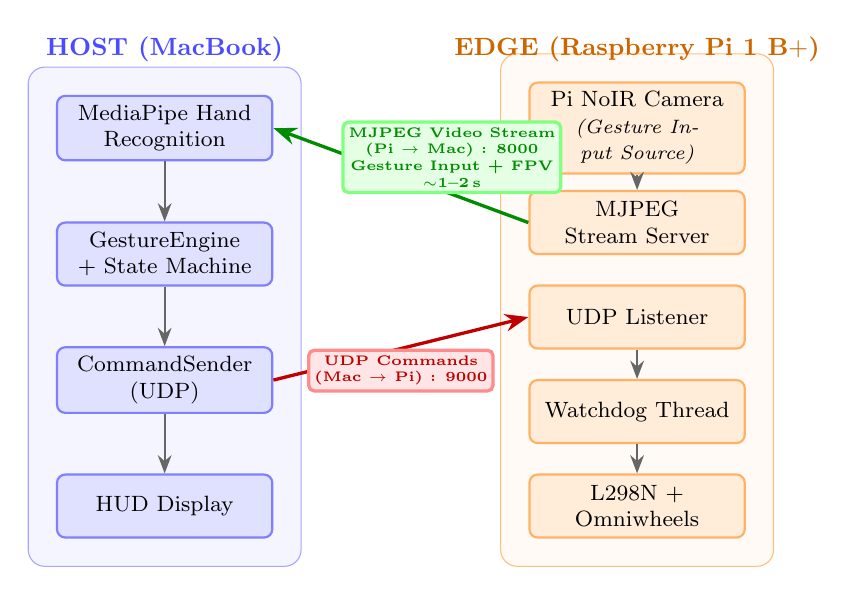
\begin{tikzpicture}[
  node distance=0.8cm,
  every node/.style={font=\footnotesize},
  box/.style={rectangle, rounded corners=3pt,
              text width=2.5cm, minimum height=0.8cm,
              align=center, draw=black!70, thick,
              fill=white},
  host/.style={box, fill=blue!12, draw=blue!50},
  edge/.style={box, fill=orange!15, draw=orange!60},
  lbl/.style={font=\bfseries\small},
  arrow/.style={-Stealth, thick, draw=black!60},
  xarrow/.style={-Stealth, very thick},
]

%% ── Column positions ──────────────────────────────────
\def\hx{0}    % host column x
\def\ex{6.0}  % edge column x

%% ── HOST nodes (top → bottom) ─────────────────────────
\node[host] (mediapipe) at (\hx, 4.0) {MediaPipe Hand Recognition};
\node[host] (gesture)   at (\hx, 2.4) {GestureEngine + State Machine};
\node[host] (sender)    at (\hx, 0.8) {CommandSender (UDP)};
\node[host] (display)   at (\hx,-0.8) {HUD Display};

%% ── EDGE nodes (top → bottom) ─────────────────────────
\node[edge, align=center] (picam) at (\ex, 4.0)
  {Pi NoIR Camera\\{\scriptsize\itshape (Gesture Input Source)}};
\node[edge] (stream)    at (\ex, 2.8) {MJPEG Stream Server};
\node[edge] (udp)       at (\ex, 1.6) {UDP Listener};
\node[edge] (watchdog)  at (\ex, 0.4) {Watchdog Thread};
\node[edge] (motors)    at (\ex,-0.8) {L298N + Omniwheels};

%% ── Column labels ─────────────────────────────────────
\node[lbl, blue!70]          at (\hx, 5.0) {HOST (MacBook)};
\node[lbl, orange!80!black]  at (\ex, 5.0) {EDGE (Raspberry Pi 1 B$+$)};

%% ── HOST internal arrows ──────────────────────────────
\draw[arrow] (mediapipe) -- (gesture);
\draw[arrow] (gesture)   -- (sender);
\draw[arrow] (sender)    -- (display);

%% ── EDGE internal arrows ──────────────────────────────
\draw[arrow] (picam)    -- (stream);
\draw[arrow] (udp)      -- (watchdog);
\draw[arrow] (watchdog) -- (motors);

%% ── Cross-network arrows ──────────────────────────────
% RED: UDP command uplink, Mac -> Pi, port 9000
\draw[xarrow, red!75!black] (sender.east) -- (udp.west)
  node[pos=0.5, below, font=\tiny\bfseries,
       fill=red!10, draw=red!45, rounded corners=2pt,
       inner sep=2pt, align=center]
       {UDP Commands\\(Mac $\rightarrow$ Pi) : 9000};

% GREEN: MJPEG video downlink, Pi -> Mac, port 8000
\draw[xarrow, green!55!black] (stream.west) -- (mediapipe.east)
  node[pos=0.3, above, font=\tiny\bfseries,
       fill=green!10, draw=green!50, rounded corners=2pt,
       inner sep=2pt, align=center]
       {MJPEG Video Stream\\(Pi $\rightarrow$ Mac) : 8000\\Gesture Input + FPV\\{\tiny $\sim$1--2\,s}};

%% ── Background panels ─────────────────────────────────
\begin{pgfonlayer}{background}
  \node[draw=blue!35, fill=blue!4, rounded corners=6pt,
        fit=(mediapipe)(gesture)(sender)(display),
        inner sep=10pt] {};
  \node[draw=orange!50, fill=orange!4, rounded corners=6pt,
        fit=(picam)(stream)(udp)(watchdog)(motors),
        inner sep=10pt] {};
\end{pgfonlayer}

\end{tikzpicture}
\end{document}
